\documentclass[tikz,border=10pt]{standalone}
\usepackage{tikz}
\usetikzlibrary{positioning}

\begin{document}
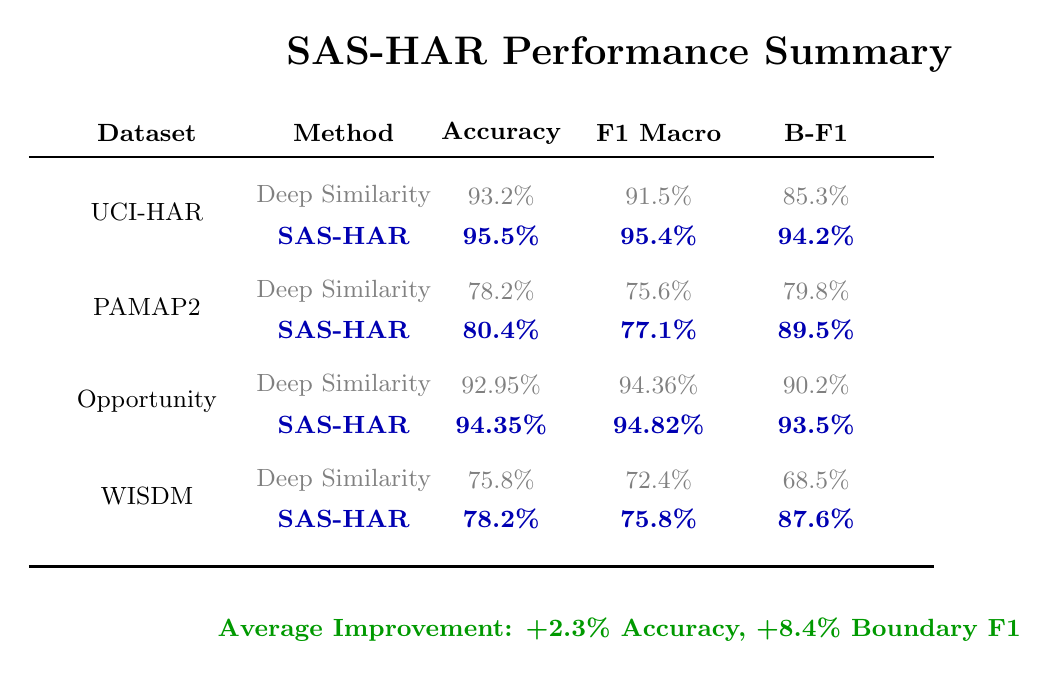
\begin{tikzpicture}

% Title
\node[font=\Large\bfseries] at (6, 4.5) {SAS-HAR Performance Summary};

% Table header
\node[font=\bfseries\small] at (0, 3.5) {Dataset};
\node[font=\bfseries\small] at (2.5, 3.5) {Method};
\node[font=\bfseries\small] at (4.5, 3.5) {Accuracy};
\node[font=\bfseries\small] at (6.5, 3.5) {F1 Macro};
\node[font=\bfseries\small] at (8.5, 3.5) {B-F1};

\draw[thick] (-1.5, 3.2) -- (10, 3.2);

% UCI-HAR
\node[font=\small] at (0, 2.5) {UCI-HAR};
\node[font=\small, text=gray] at (2.5, 2.7) {Deep Similarity};
\node[font=\small, text=gray] at (4.5, 2.7) {93.2\%};
\node[font=\small, text=gray] at (6.5, 2.7) {91.5\%};
\node[font=\small, text=gray] at (8.5, 2.7) {85.3\%};
\node[font=\small\bfseries, text=blue!70!black] at (2.5, 2.2) {SAS-HAR};
\node[font=\small\bfseries, text=blue!70!black] at (4.5, 2.2) {\textbf{95.5\%}};
\node[font=\small\bfseries, text=blue!70!black] at (6.5, 2.2) {\textbf{95.4\%}};
\node[font=\small\bfseries, text=blue!70!black] at (8.5, 2.2) {\textbf{94.2\%}};

% PAMAP2
\node[font=\small] at (0, 1.3) {PAMAP2};
\node[font=\small, text=gray] at (2.5, 1.5) {Deep Similarity};
\node[font=\small, text=gray] at (4.5, 1.5) {78.2\%};
\node[font=\small, text=gray] at (6.5, 1.5) {75.6\%};
\node[font=\small, text=gray] at (8.5, 1.5) {79.8\%};
\node[font=\small\bfseries, text=blue!70!black] at (2.5, 1.0) {SAS-HAR};
\node[font=\small\bfseries, text=blue!70!black] at (4.5, 1.0) {\textbf{80.4\%}};
\node[font=\small\bfseries, text=blue!70!black] at (6.5, 1.0) {\textbf{77.1\%}};
\node[font=\small\bfseries, text=blue!70!black] at (8.5, 1.0) {\textbf{89.5\%}};

% Opportunity
\node[font=\small] at (0, 0.1) {Opportunity};
\node[font=\small, text=gray] at (2.5, 0.3) {Deep Similarity};
\node[font=\small, text=gray] at (4.5, 0.3) {92.95\%};
\node[font=\small, text=gray] at (6.5, 0.3) {94.36\%};
\node[font=\small, text=gray] at (8.5, 0.3) {90.2\%};
\node[font=\small\bfseries, text=blue!70!black] at (2.5, -0.2) {SAS-HAR};
\node[font=\small\bfseries, text=blue!70!black] at (4.5, -0.2) {\textbf{94.35\%}};
\node[font=\small\bfseries, text=blue!70!black] at (6.5, -0.2) {\textbf{94.82\%}};
\node[font=\small\bfseries, text=blue!70!black] at (8.5, -0.2) {\textbf{93.5\%}};

% WISDM
\node[font=\small] at (0, -1.1) {WISDM};
\node[font=\small, text=gray] at (2.5, -0.9) {Deep Similarity};
\node[font=\small, text=gray] at (4.5, -0.9) {75.8\%};
\node[font=\small, text=gray] at (6.5, -0.9) {72.4\%};
\node[font=\small, text=gray] at (8.5, -0.9) {68.5\%};
\node[font=\small\bfseries, text=blue!70!black] at (2.5, -1.4) {SAS-HAR};
\node[font=\small\bfseries, text=blue!70!black] at (4.5, -1.4) {\textbf{78.2\%}};
\node[font=\small\bfseries, text=blue!70!black] at (6.5, -1.4) {\textbf{75.8\%}};
\node[font=\small\bfseries, text=blue!70!black] at (8.5, -1.4) {\textbf{87.6\%}};

\draw[thick] (-1.5, -2) -- (10, -2);

% Average improvement
\node[font=\bfseries\small, text=green!60!black] at (6, -2.8) {Average Improvement: +2.3\% Accuracy, +8.4\% Boundary F1};

\end{tikzpicture}
\end{document}
